\chapter{On-Body Device}
The on-body device was developed by William Tran in 2022~\cite{Tran:2022} and consists of
a PIC32 as the primary microcontroller and an ESP32 acting as a wireless bridge,
as well as ADS1294R 24-bit analog-to-digital converter for taking biosignal measurements.

The ESP32 had been programmed to connect to WiFi, but was only programming intermittently,
and the WiFi connection was reported but no data had been written or received.

The only other contributions were from Craig Dawson who supplied information and boilerplate code for programming the PIC32,
as well as attaching wires to specific pins of the PIC32, allowing it to be probed using an oscilloscope.


\section{Methods}
The previously programmed ESP32 was verified to determine if data would be able to be sent via WiFi.
During this process, inconsistencies in programming were discovered.
Over-the-air updates~\cite{Quadri:2014} were implemented to make programming more consistent.
Then, the device was connected to the off-body PC wirelessly.

The PIC32 was programmed with a basic test program.
Then, PLL~\cite{Maji:2016} clock configuration was performed and validated.

SPI communication between the PIC32 and the ESP32 was established.
Further communication between the PIC32 and the off-body PC through the ESP32 was verified.
The ADS1294R communication line was probed, and SPI communication was briefly established with the PIC32.

Issues surrounding the ADS1294R prompted an investigation into the power distribution of the on-body PCB.
Additionally, further issues had arose surrounding power into the ESP32.
The PCB was tested in the following states in order to measure changes in how the ESP32 programmed.

\begin{itemize}
        \item The board was connected to a lab bench power supply with a non-restrictive current limit.
        \item The boot select switch was held for the extent of the programming cycle.
        \item The boot select switch was held until programming began.
        \item The boot select switch was held from when the device was powered on until programming ended.
        \item The board was powered from a lab bench power supply as well as via USB through an ICD 3.
        \item All the same boot select switch options were repeated with the additional power being supplied.
\end{itemize}


\section{Results}
The ESP32 had a programming consistency of less than 50\%.
After over-the-air updates were implemented, the board successfully received updates more than 90\% of the time.
The remaining programming inconsistencies come from power supply issues as will be addressed later in this section.

The ESP32 is able to connected to the network and can wirelessly transmit arbitrary bytes of data to the off-body PC consistently at 1 MB/s.

The PIC32 was configured with an 80 MHz system clock and is able to be put into hardware debugging mode.
The clock has been verified using an oscilloscope to measure the time between pin changes using blocking delays,
this can be seen in~\autoref{image:pulse_delay}.

\begin{figure}[!ht]
  \caption{Oscilloscope measurement of 100ms delay between pulses}\label{image:pulse_delay}
  \centering
  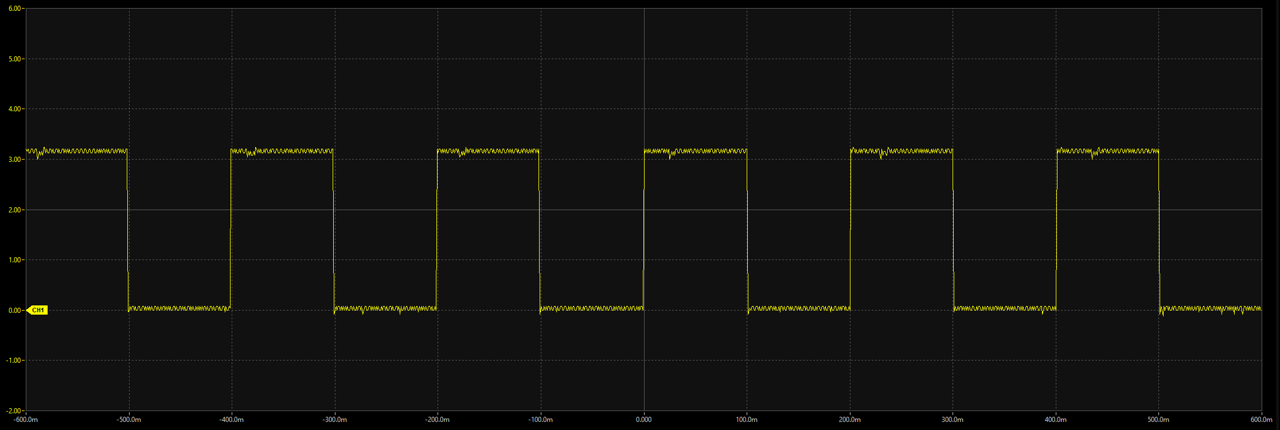
\includegraphics[width=1\columnwidth]{chapters/development/results/DELAY}
\end{figure}

The PIC32 and ESP32 are able to communicate with 0 bit rate errors over a half hour runtime.
However, the communication has a number of required delays that should be optimized in the future.
This limits the overall system communication speed substantially.

Communication between the ADS1294R and the PIC32 worked, and test signals from the ADS1294R were measured.
This communication did not last long enough to substantially test, as the PCB began to have power issues.

The voltage at the input of the ESP32 was 0.7 V less than what was measured at the input power supply (3.3 V).
The input power supply was not reaching it's current limit.
Changing the boot select pin did not make a difference in the way that the ESP32 was programmed, until the additional power supply was added.
Adding the power supply made the voltage at the ESP32 higher, around 3.1 V.
This allows it to be programmed, but it is not completely consistent as sometimes the voltage drops low enough that the device resets.


\section{Discussion}
The inconsistencies regarding the ESP32 programming all revolve around unintentional resetting of the device due to low voltage.
When the device is being programmed using the hardware programmer, the device needs to be put into the programming boot mode.
To do this, the boot switch should be held down as the device is powered on. Then, once the device is on, the boot switch can be released.
In normal operation, the device would stay in programming mode until it is either programmed or reset.
However, in this circuit, the ESP32 is often reset due to brownout detection, such a reset can be seen in~\autoref{fig:brownout}.

\begin{figure}[!ht]
  \caption{ESP32 brownout detection example}\label{fig:brownout}
  \centering
  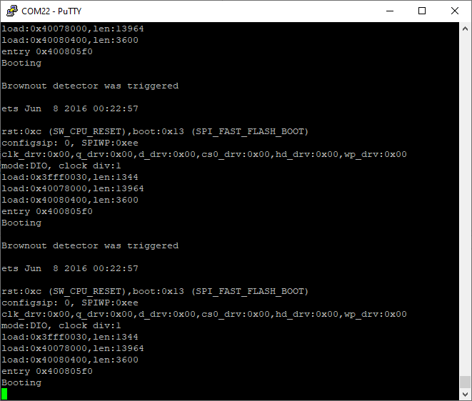
\includegraphics[width=\textwidth/2]{chapters/development/brownout_detection}
\end{figure}

This reset would either cause the device to reset again,
due to the sudden draw of current of the device turning on being enough to drop the voltage to the point where it would turn off again,
or if it did manage to turn on, no longer be in programming mode.
Additionally, to get the ESP32 into programming mode required the PCB to be completely unpowered
so that the switch could be held as it is powered again.
This would also cause issues as all the devices on the PCB would power on at the same time and often the ESP32 would reset at this point,
requiring the entire process to be repeated.

The implementation of over-the-air programming fixed the inconsistencies because it does not require the ESP32 to be put into programming mode.
This means that the PCB can be powered consistently and all devices can be powered on completely, with only the ESP32 resetting due to the programming.
Which is a lot less likely to cause a substantial voltage drop and trip the brownout detection of the ESP32.

The PIC32 programming was challenging because the device was not correctly labelled on the schematics.
Due to chip shortages during manufacturing, a different model of PIC32 had to be chosen, however this was not obviously reflected in the schematics.
This meant that the intial implemention of the PIC32 revolved around attempting to connect to a device with a different device ID.

Communication between the PIC32 and the ESP32 was done with SPI.
SPI is typically used between a controller and a peripheral.
In this case, the PIC32 would be the controller, and the ESP32 would be the wireless transmitter `peripheral'.
However, since both devices are microcontrollers, both devices are configured to be the controller.
In order to make the ESP32 the controller,
it would need to be continuously sending dummy data in order to generate the clock pulses for the PIC32 to send data,
which is unoptimal for this use case as the PIC32 is only ever sending data and the ESP32 is only ever receiving it.
So, it makes more sense to make the PIC32 the controller.

The library that was used to make the ESP32 act as an SPI peripheral is the ESP32DMASPI library~\cite{ESP32DMASPI}.
This library is based on the official driver from the manufacture~\cite{SPI}.
SPI was implemented using task based DMA receiving.
The PIC32 is configured as a 32-bit master operating in SPI mode 3~\cite{Barry:2012}.
The baudrate generator value has been calculated using the equation \(BRG = (F_{PB} / 2 \times F_{SCK}) - 1\),
and a SPI clock speed of 31.3 kHz has been generated (using a BRG value of 50).
This value has been intentionally set low so that the transmission speeds are well below what both devices are capable of for testing.

An additional delay is required between SPI writes in order to stop data from becoming corrupt.
This delay was embedded into the low-level driver to make eventual performance optimization centralized,
since this delay is a clear cost to performance and by far the cause of the most communication slowdown.
This delay is most likely necessary due to the operation of the SPI chip select line.
Specifically, the way the chip select line does not reset between SPI transmissions without adequate delays between writes.
This could be solved by manually asserting the chip select line instead of allowing the peripheral to control it.
However, due to time restrictions it was decided that features should be implemented in a basic functional form,
and performance could be optimized once the system was fully developed,
and thus the driver was implemented using significantly slower delay.

The ADS1294R also communicates using SPI.
A recommended startup sequence for the device is shown in~\autoref{fig:ads_startup}.
When first communicating with the device, this startup sequence was followed as closely as possible.

\begin{figure}[!ht]
  \caption{ADS1294R startup sequence}\label{fig:ads_startup}
  \centering
  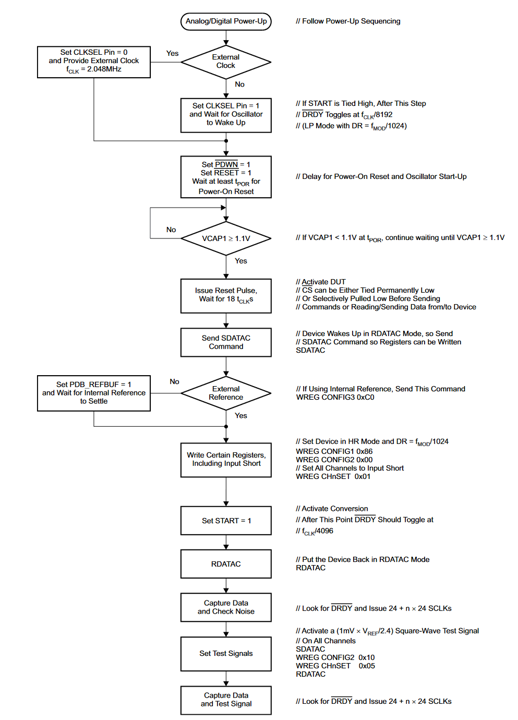
\includegraphics[width=1\columnwidth/2]{chapters/development/results/ADS_Startup_Sequence}
\end{figure}

However, the device did not operate as expected.
No matter what command the device was given, it would continually output the same byte.
The byte did not correlate to the ID of the device, and it did not appear to change, regardless of what commands were sent to the device.

The only commands that the device did respond to were single byte commands.
But because the device was responding to the commands, it proved that the communication must work in at least one direction.
Still, to aid in troubleshooting, debugging wires were attached to the board, shown in~\autoref{fig:pic_wires}.

\begin{figure}[!ht]
  \caption{PIC32 board attached debugging wires}\label{fig:pic_wires}
  \centering
  \includegraphics[width=1\columnwidth]{chapters/development/results/P_20230919_170532}
\end{figure}

A four channel oscilloscope could then be used to analyze the SPI communication.
What was eventually discovered was that the chip select pin was not being asserted for long enough.
The SPI communication between the two devices is shown in~\autoref{fig:ads_spi}.
Since the chip select pin was being controlled by the PIC SPI module,
it was being automatically driven low during transmission and then high again after transmission completed.
For multi-byte commands the chip select line needed to stay asserted until all of the bytes had been transferred and received.
That is why it would only work for single-byte commands, because once the byte had been send the communication could be reset.

\begin{figure}[!ht]
  \caption{SPI communication between PIC32 and ADS1294R}\label{fig:ads_spi}
  \centering
  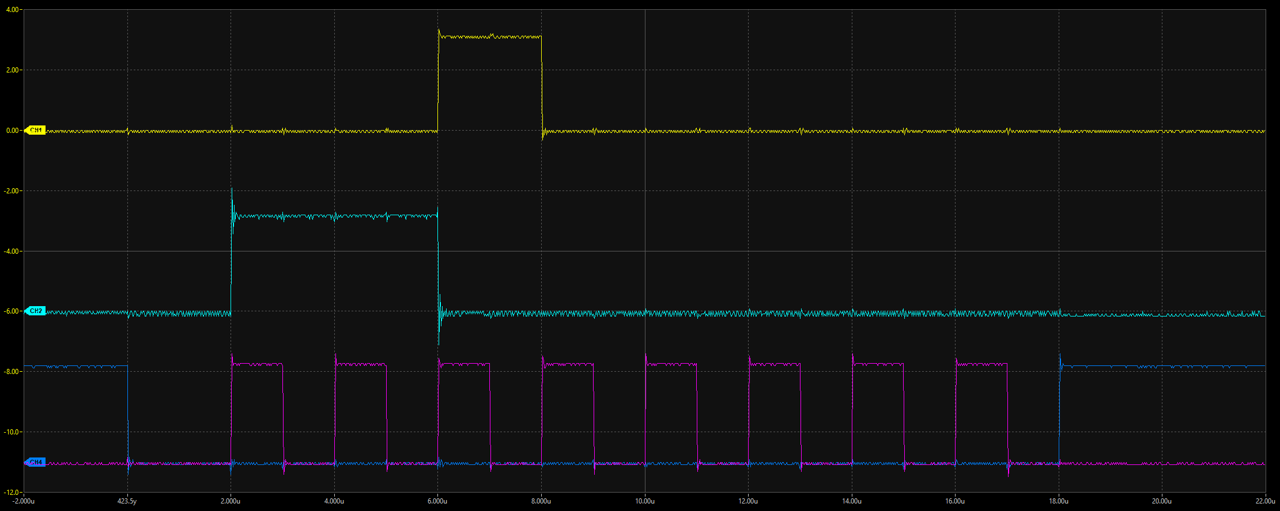
\includegraphics[width=1\columnwidth]{chapters/development/results/ADS_SPI_COMMS}
\end{figure}

The board power distribution issues arose once the SPI communication between the PIC32 and the ADS1294R had been established.
There are a number of possibilities for why this would happen.

The first possibility that was invested was the addition of the attached debugging wires, as they may have created a short circuit.
However, none of the adjacent pins of any of the debugging wires were power related,
nor were they electrically connected as measured using the continuity test function of a multimeter.

Another possibility is that the voltage regulator and/or power source are not rated to high enough current.
To verify this was not the cause, the voltage regulator was bypassed and the board was directly driven by the source power supply,
the feasibility of this was determined by referencing the board schematics.
The current limit of the source supply was also increased so that it remained in constant voltage mode,
and was monitored to determine that the current limit was never reached.

The final possibility that was investigated was the increase in current draw from all of the integrated circuits now being functional.
As the resistance of the power plane of the board is constant,
the equation \[V = IR\] tells us that an increase in current will cause a proportional increase in voltage drop across the power plane.
If the resistance of the power plane is high enough, and the current increase great enough,
it is possible that the voltage across the power plane could trigger the brownout detection, or other undefined behaviour, for some of the devices.
If this caused a number of devices to reset at the same time, it may cause a peak in current consumption at the point were they all startup again.
This would cause a greater voltage drop across the power plane, thus repeating the cycle.
One attempt to circumvent this was to insert power into a number of different points on the board
closer to where the supply pins of the integrated circuit are.
This had some brief success, but ultimately did not provide a consistent method for keeping the device powered correctly,
as the devices would intermittently reset due to power issues.
It appeared that the only way to keep the board powered consistently was to keep the debugging tools for each device connected permanently,
and to power each device through its corresponding debugger.

This implies that the issues are more related to the source supply rather than the power plane.
However, each individual debugger is not able to power the board without it having the same issue.
Additionally, several debuggers in parallel still do not solve the issue.
It is only the addition of the debugging tools and the source supply that solve the issue.
With the debugging tools disconnected, the source supply current reading increases.
So, the additions do not provide power that the source supply is unable to supply itself.
Unfortunately, due to time constraints, no further investigation could be conducted.
